\documentclass[aspectratio=169]{beamer}

\usetheme{default}

\usepackage[utf8]{inputenc}
\usepackage[russian]{babel}
\usepackage[OT1]{fontenc}
\usepackage{amsmath}
\usepackage{amsfonts}
\usepackage{amssymb}
\usepackage{graphicx}
\usepackage{etoolbox}
\usepackage{caption}
\usepackage{subcaption}
\captionsetup{compatibility=false}
\usepackage{pifont}
%\usepackage{subfigure}
\usepackage{xcolor}
\usepackage{framed}
\usepackage{empheq}
\usepackage[many]{tcolorbox}
\usepackage{multirow}
\usepackage{tikz}
\usepackage{listings}
\usepackage{tikz}

\definecolor{shadecolor}{cmyk}{0,0,0,1}

\lstset{
	backgroundcolor=\color{lightgray},
	commentstyle=\color{blue},
	frame=single
	breakatwhitespace, 
	language=python, 
	columns=fullflexible, 
	keepspaces, 
	breaklines, 
	tabsize=3, 
	showstringspaces=false, 
	extendedchars=true,
	numbers=left
}

\makeatletter

\setbeamercolor{title}{fg=white}
\setbeamercolor{frametitle}{fg=black}
\setbeamerfont*{title}{family=\sffamily,size=\LARGE}

\setbeamerfont{page number in head/foot}{size=\scriptsize}
\setbeamertemplate{footline}[frame number]
\let\otp\titlepage
\renewcommand{\titlepage}{\otp\addtocounter{framenumber}{-1}}

\setbeamertemplate{background canvas}{%
	\ifnumequal{\c@framenumber}{0}{%
		\vbox to \paperheight{\vfil\hbox to \paperwidth{\hfil
\includegraphics[height=\paperheight]{images/cover.png}\hfil}\vfil}
   }{%
      \ifnumequal{\c@framenumber}{\inserttotalframenumber}{
        \vbox to \paperheight{\vfil\hbox to \paperwidth{\hfil
\includegraphics[height=\paperheight]{images/back.png}\hfil}\vfil}
      }{%
         % Other frames
      }%
   }%
}

\makeatother

\beamertemplatenavigationsymbolsempty

\tcbset{highlight math style={enhanced,colframe=red,colback=white,arc=4pt,boxrule=1pt}}

\usetikzlibrary{shadings,shadows,shapes.arrows}

\newcommand*{\tikzarrow}[2]{%
  \tikz[
    baseline=(A.base),             % Set baseline to the baseline of node content
    font=\footnotesize\sffamily    % Set fontsize of the node content
  ]
  \node[
    single arrow,                  % Shape of the node
    single arrow head extend=5pt,  % Actual width of arrow head
    draw,                          % Draw the node shape
    inner sep=3pt,                 % Separation between node content and node shape
    top color=#1,               % Shading color on top of node
    bottom color=#1,               % Shading color on bottom of node
    % drop shadow                    % Draw a shadow
  ] (A) {#2};%
}

\newcommand{\tikzfancyarrow}[2][2cm]{\tikz[baseline=-0.5ex]\node [arrowstyle=#1] {#2};}
\newcommand*\rot{\rotatebox{90}}

\author{Николай Анохин}
\title{\newline \newline \newline Лекция 3 \\ Алгоритмы кластеризации II}

\begin{document}

\begin{frame}[plain]
\titlepage
\end{frame}

\begin{frame}{Краткое содержание предыдущих лекций}

\vspace{1em}
{\bf Дано.} Признаковые описания $N$ объектов $\mathbf{x} = (x_1, \ldots, x_m) \in \mathcal{X}$, образующие тренировочный набор данных $X$

\vspace{1em}
{\bf Найти.} Модель из семейства параметрических функций 
\[
H = \{h(\mathbf{x, \mathbf{\theta}}): \mathcal{X} \times \Theta \rightarrow \mathcal{Y} \mid \mathcal{Y} = \{1, \ldots, K\}\},
\]
ставящую в соответствие произвольному $\mathbf{x} \in \mathcal{X}$ один из $K$ кластеров так, чтобы объекты внутри одного кластера были похожи, а объекты из разных кластеров различались

\end{frame}

\begin{frame}{Краткое содержание предыдущих лекций}

\begin{columns}[]
    \begin{column}{.4\textwidth}
    	Рассмотрели классические алгоритмы кластеризации
		\begin{enumerate}
			\item Смесь гауссовских распределений и k-means++
			\item Hierarchical Clustering
			\item DBSCAN
		\end{enumerate}    	
		И как их использовать
		\begin{enumerate}
			\item Выбор количества кластеров
			\item Оценка качества
		\end{enumerate}
		
    \end{column}
       
    \begin{column}{.6\textwidth}
    \vspace{-0em}
	\begin{center}
   		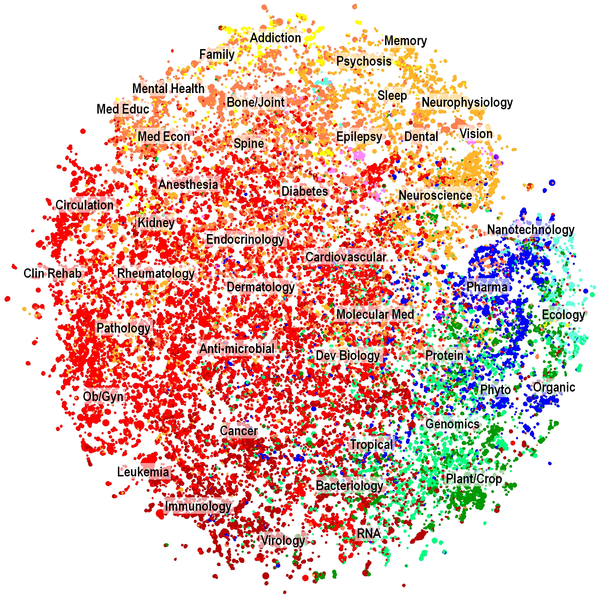
\includegraphics[width=\textwidth]{images/medical.png}
    \end{center}
    \end{column}
  \end{columns}

\end{frame}

% ============================================== %

\section{Кластеризация больших данных}

% ============================================== %

\begin{frame}

\begin{center}
{\Large Кластеризация больших данных\footnote{\href{http://www.researchgate.net/publication/276934256_Big_Data_Clustering_Algorithms_and_Challenges}{Big Data Clustering: Algorithms and Challenges}}}

\vspace{2em}
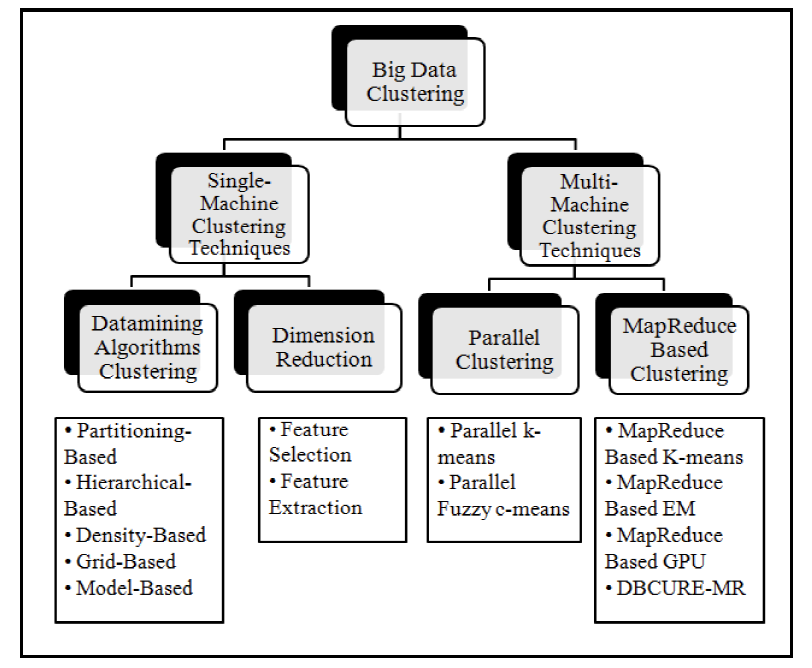
\includegraphics[height=0.6\textheight]{images/bdc.png}
\end{center}

\end{frame}

\begin{frame}{Balanced Iterative Reducing and Clustering using Hierarchies (BIRCH)\footnote{\href{http://www.cs.sfu.ca/CourseCentral/459/han/papers/zhang96.pdf}{BIRCH: An efficient data clustering method for very large datasets}}}

{\it Идея метода:} построить иерархию кластеров, которая позволит хранить ограниченное количество данных в виде агрегатов.

\vspace{1em}
\begin{itemize}
\item {\it локальность:} каждая точка ``кластеризуется'' без сканирования всех других точек или имеющихся кластеров
\item {\it выбросы:} точки в ``густонаселенных'' регионах принадлежат кластерам, а в ``малонаселенных'' --  к выбросам 
\item {\it экономность:} используется вся доступная память, при этом минимизируется I/O
\item {\it масштабируемость:} при определенных условиях обучается ``онлайн'' и требует единственного прохода по данным
\end{itemize}

\end{frame}

\begin{frame}{Меры компактности кластера}

Центроид
\[
\mathbf{x}_0 = \frac{1}{N} \sum_{i=1}^N \mathbf{x}_i
\]
Радиус
\[
R = \frac{1}{N} \sum_{i=1}^N d(\mathbf{x}_i, \mathbf{x}_0)
\]
Диаметр
\[ 
\quad D = \frac{1}{N(N-1)} \sum_{i=1}^N \sum_{j=1}^N d(\mathbf{x}_i, \mathbf{x}_j)
\]

\end{frame}

\begin{frame}{Clustering Feature}

Clustering feature -- это объект, содержащий сжатую информацию о кластере.

\vspace{1em}
\begin{block}{Определение 1}
Пусть кластер $C$ содержит $N$ $d$-мерных объектов $\mathbf{x}_i$. Clustering feature (CF) для $C$ определяется как тройка $CF = (N, LS, SS)$, где 
\[
LS = \sum_{i=1}^N \mathbf{x}_i, \quad SS = \sum_{i=1}^N \mathbf{x}^2_i
\]
\end{block}
\begin{block}{Утверждение 1}
Пусть $CF_1 = (N_1, LS_1, SS_1)$ и $CF_2 = (N_2, LS_2, SS_2)$ -- CF для кластеров $C_1$ и $C_2$. Тогда CF для кластера, полученного слиянием $C_1$ и $C_2$, определяется как
\[
CF = (N_1 + N_2, LS_1 + LS_2, SS_1 + SS_2)
\]

\end{block}

\end{frame}

\begin{frame}{CF Tree}

B --  максимальное количество детей у внутреннего узла \\
L -- максимальное количество детей у листа \\
T -- Максимальная компактность ($R$ или $D$) ребенка листа

\begin{columns}[]
  \begin{column}{.6\textwidth}
  \begin{center}
   		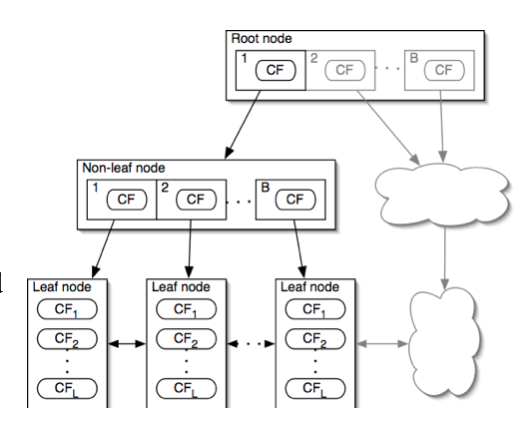
\includegraphics[height=0.7\textheight]{images/cftree.png}
    \end{center}
		
  \end{column}       
  \begin{column}{.4\textwidth}
  При разделении узла выбираем две наиболее удаленные CF и	лепим к ним ближайшие
  \end{column}
\end{columns}

\end{frame}

\begin{frame}{BIRCH}

\begin{center}
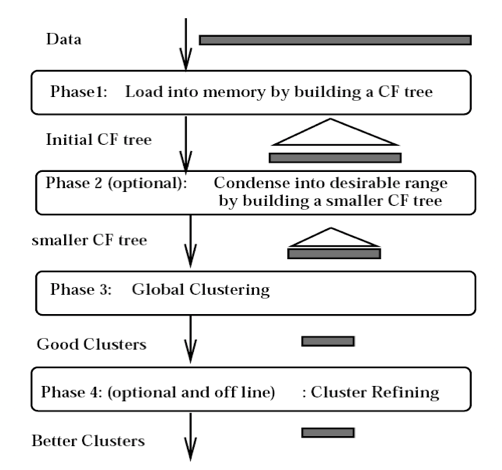
\includegraphics[height=0.9\textheight]{images/birch.png}
\end{center}

\end{frame}

\begin{frame}{Пример}

\begin{center}
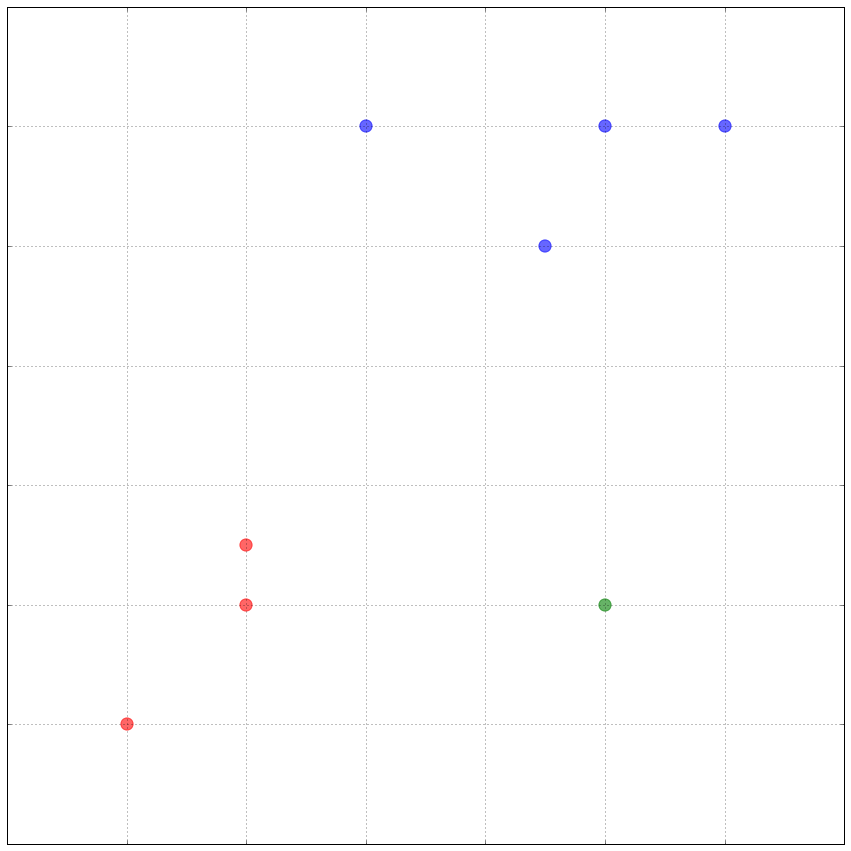
\includegraphics[height=0.9\textheight]{images/toy.png}
\end{center}

\end{frame}

\begin{frame}[fragile]{Сравнение скорости}

\begin{center}
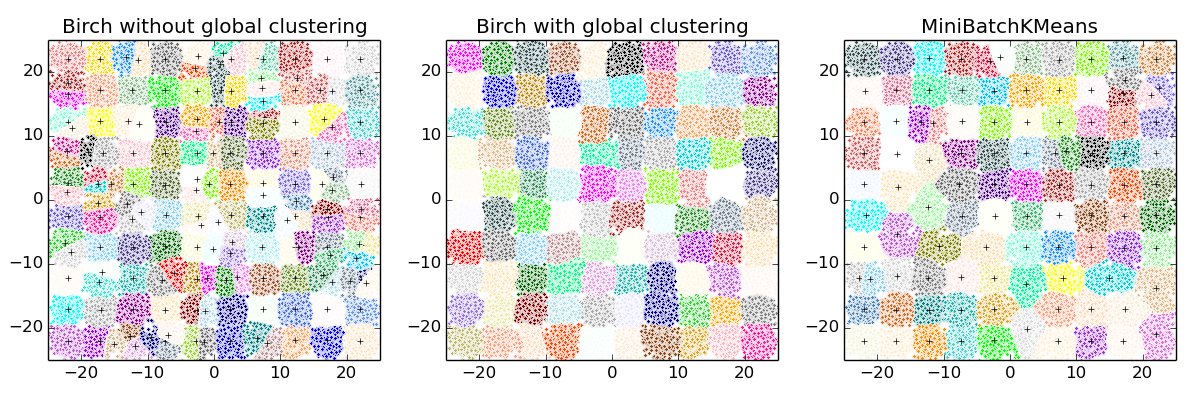
\includegraphics[width=0.9\textwidth]{images/compare.png}
\end{center}

\begin{verbatim}
Birch without global clustering as the final step took 4.19 seconds
n_clusters : 158
Birch with global clustering as the final step took 4.61 seconds
n_clusters : 100
Time taken to run MiniBatchKMeans 5.61 seconds
\end{verbatim}

\end{frame}

\begin{frame}{Итоги}

\begin{itemize}
\item[+] Алгоритм работает за $O(N)$
\item[+] Можно контролировать количество используемой памяти
\item[+] В некоторых случаях поддерживается онлайн кластеризация
\item[--] Тяжелый подбор параметров
\item[--] Только эллиптические кластеры
\end{itemize}

\end{frame}

\begin{frame}{Другие алгоритмы\footnote{\href{http://bib.dbvis.de/uploadedFiles/176.pdf}{DENCLUE}}\footnote{\href{http://fusion.cs.uni-magdeburg.de/pubs/optigrid.pdf}{OptiGrid}}\footnote{\href{https://www.wikiwand.com/en/Fuzzy_clustering}{Fuzzy c-means}}}

\begin{center}
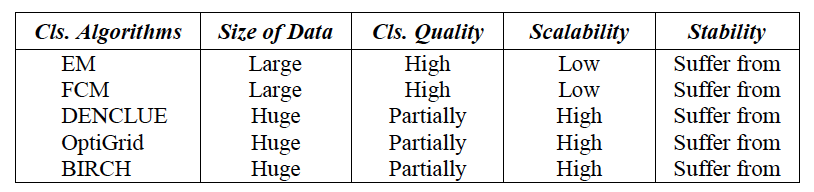
\includegraphics[width=0.9\textwidth]{images/summary.png}
\end{center}

\end{frame}

% ============================================== %

\section{Multidimensional Scaling}

% ============================================== %

\begin{frame}

\begin{center}
{\Large Multidimensional Scaling}

\vspace{1em}

\includegraphics[width=0.8\textwidth]{images/curse.png}
\end{center}

\end{frame}

\begin{frame}{Идея метода}

Перейти в пространство меньшей размерности так, чтобы расстояния между объектами в новом пространстве были подобны расстояниям в исходном пространстве.

\end{frame}

\begin{frame}{t-Stochastic Neighbour Embedding (t-SNE)\footnote{\url{http://lvdmaaten.github.io/tsne/}}}

Схожесть между объектами в исходном пространстве
\[
p(i, j) = \frac{p(i | j) + p(j | i)}{2n}, \quad p(j | i) = \frac{\exp(-\|\mathbf{x}_j-\mathbf{x}_i\|^2/{2 \sigma_i^2})}{\sum_{k \neq i}\exp(-\|\mathbf{x}_k-\mathbf{x}_i\|^2/{2 \sigma_i^2})}
\]
Схожесть между объектами в целевом пространстве
\[
q(i, j) = \frac{(1 + \| \mathbf{y}_i - \mathbf{y}_j \|^2)^{-1}}{\sum_{k \neq l}(1 + \| \mathbf{y}_k - \mathbf{y}_l \|^2)^{-1}}
\]
Критерий
\[
J_{t-SNE} = KL(P \| Q) = \sum_i \sum_j p(i, j) \log \frac{p(i, j)}{q(i, j)} \rightarrow \min
\]

\end{frame}

\begin{frame}{t-распределение}

\[
\tau(\mu, \sigma^2, \nu) \propto \left[1 + \frac{1}{\nu}\left(\frac{x-\mu}{\sigma}\right)^2\right]^{-\frac{\nu+1}{2}}
\]

\begin{center}
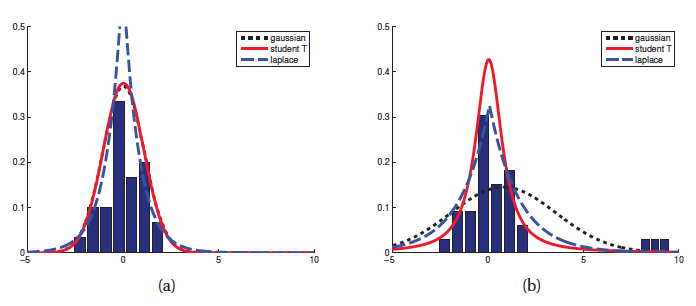
\includegraphics[scale=0.4]{images/t-distr.png}
\end{center}

Уильям Госсет 1908 (Student)

\end{frame}

\begin{frame}{Дивергенция Кульбака-Лейблера}

Насколько распределение $P$ отличается от распределения $Q$?
\[
KL(P \| Q) = \sum_z P(z) \log \frac{P(z)}{Q(z)}
\]

\end{frame}

\begin{frame}{Digits Dataset}

около 1800 картинок 8x8 с рукописными цифрами 

\begin{center}
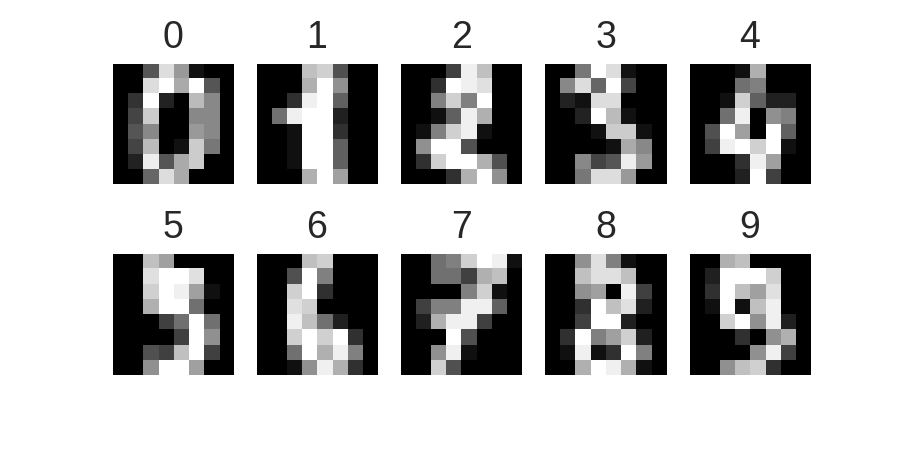
\includegraphics[scale=0.5]{images/digits.png}
\end{center}

\href{https://raw.githubusercontent.com/oreillymedia/t-SNE-tutorial/master/images/animation.gif}{t-SNE}

\end{frame}

\begin{frame}{MNIST Dataset}

70000 картинок 20x20 с рукописными цифрами 

\begin{center}
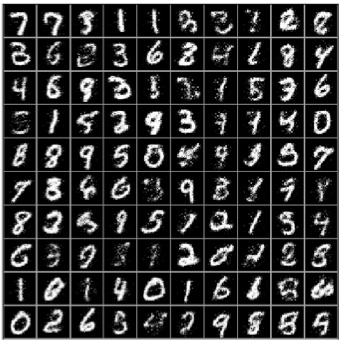
\includegraphics[scale=1.0]{images/mnistdigits.jpg}
\end{center}

\href{http://lvdmaaten.github.io/tsne/examples/mnist_tsne.jpg}{t-SNE}

\end{frame}

\begin{frame}{Еще примеры}

\href{http://lvdmaaten.github.io/tsne/examples/caltech101_tsne.jpg}{CalTech}

\vspace{1em}
\href{http://lvdmaaten.github.io/tsne/examples/SP500_tsne.png}{S\&P 500}

\vspace{1em}
\href{http://www.cs.toronto.edu/~hinton/turian.png}{Words}

\end{frame}

\begin{frame}{Еще алгоритмы}

\begin{center}
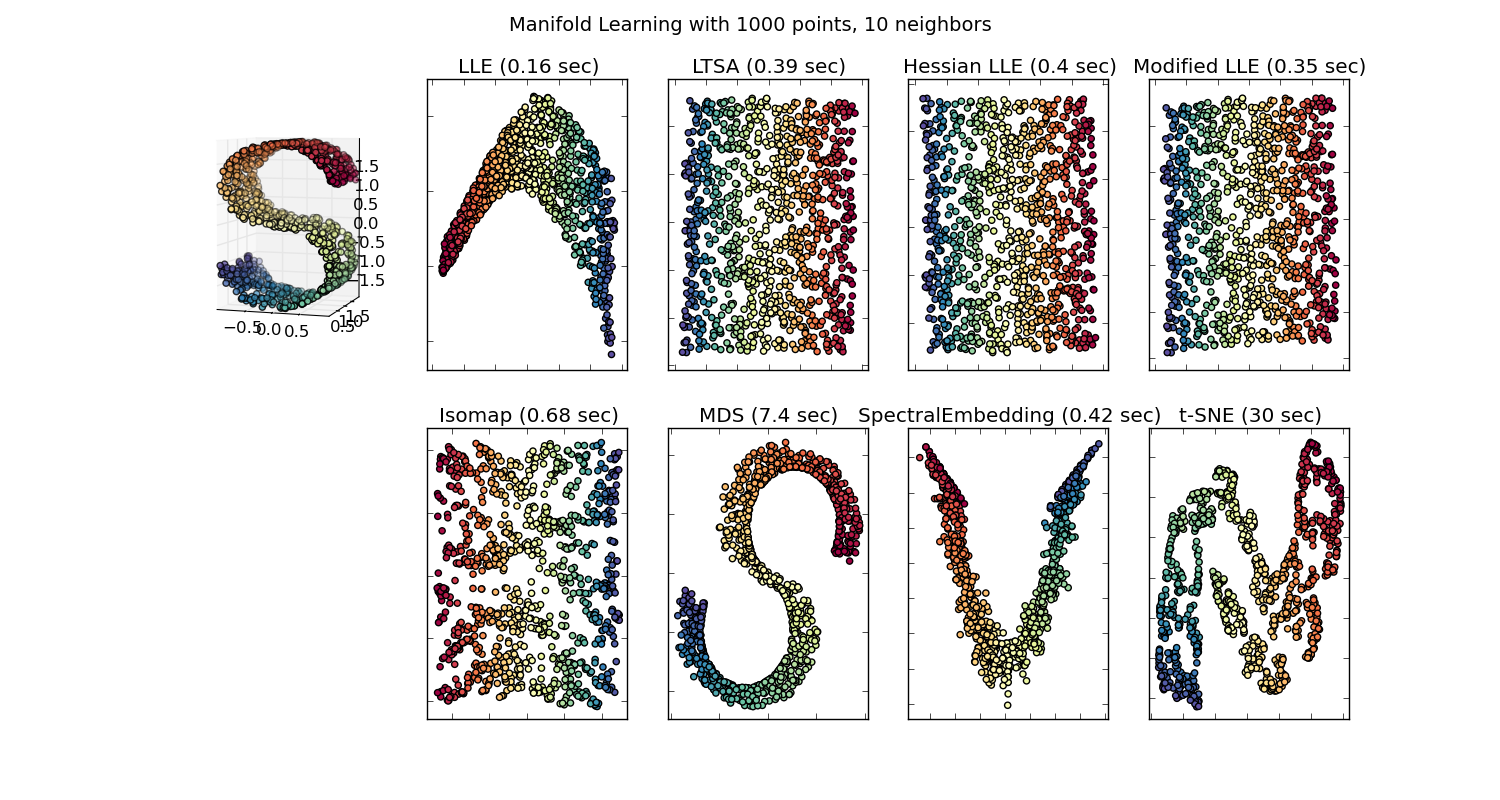
\includegraphics[scale=0.27]{images/mainfold.png}
\end{center}

\end{frame}

\begin{frame}[plain]
\begin{center}
{\Large Вопросы}
\end{center}
\end{frame}

\end{document}